\documentclass[dvipdfmx]{beamer}

\usepackage{bxdpx-beamer}
\usepackage{pxjahyper}
\usepackage{minijs}
\usepackage[T1]{fontenc}
\usepackage{lmodern}
\usepackage{xcolor}
\usepackage{textcomp}

\usepackage{amsmath, amssymb, mathtools, bm}
\usepackage{comment}

\renewcommand{\kanjifamilydefault}{\gtdefault}

\usetheme{Madrid}
\usecolortheme[RGB={32,135,185}]{structure}
\usefonttheme{professionalfonts}
\setbeamercolor{background canvas}{bg=gray!10}
% \setbeamertemplate{footline}[page number]
\setbeamertemplate{navigation symbols}{}
\setbeamertemplate{itemize item}[circle]
\setbeamertemplate{itemize subitem}[circle]
\setbeamertemplate{itemize subsubitem}[circle]
\setbeamertemplate{enumerate item}[default]



\title[Jukebox \ (Dhariwal+, 2020)]{
    Jukebox: A Generative Model for Music \\
    {\large Prafulla Dhariwal et al., 2020}
}
\author{吉永 塁}
\date{September 30, 2020}


\begin{document}

\begin{frame}[plain,noframenumbering]
    \titlepage
\end{frame}


\begin{frame}
    \frametitle{概要}
    \begin{itemize}
        \item 内容:音楽生成
        \item 特徴:
            \begin{enumerate}
                \item raw audio domain で歌を伴う音楽を生成できる
                \item 数分の長さの楽曲を生成することができる
                \item 生成時に楽曲スタイルを条件指定できる
            \end{enumerate}
        \vspace{\baselineskip}
        \item 実際に生成された楽曲 {\footnotesize \url{https://jukebox.openai.com/}}
        % \item ソースコード {\footnotesize \url{https://github.com/openai/jukebox/}}
    \end{itemize}
\end{frame}


\begin{frame}
    \frametitle{先行研究}
    \begin{itemize}
        \item 生成モデル
        \begin{itemize}
            \item 文章生成
            \item 音声生成
            \item 画像生成
        \end{itemize}
        近年急速に発展
        \vspace{\baselineskip}
        \item 音楽生成モデル
        \begin{itemize}
            \item symbolicなアプローチ
            \begin{itemize}
                \item 低次元空間上なのでモデリングが簡単
                \item 生成できる音楽に制約がかかる(例:楽器の音が固定)
            \end{itemize}
            \item non-symbolicなアプローチ
            \begin{itemize}
                \item 音楽をaudioとして直接生成
                \item raw audioは高次元で情報量が多い
                \item 長期依存性(long-range dependency)により音楽の高度な意味(semantics)の学習が難しい
            \end{itemize}
        \end{itemize}
    \end{itemize}
\end{frame}


\begin{frame}
    \frametitle{提案手法}
    重要度の低い情報を捨て,音楽の大部分の情報を保持するように圧縮

    \begin{itemize}
        \item Hierarchical VQ-VAEの構造を用いてaudioを離散空間へ圧縮
        \item priorモデルによって離散空間上でcodeを生成
        \item 生成されたcodeをVQ-VAE(Decoder)によって再構成
    \end{itemize}
\end{frame}


\begin{frame}
    \frametitle{Music VQ-VAE}
    \begin{center}
        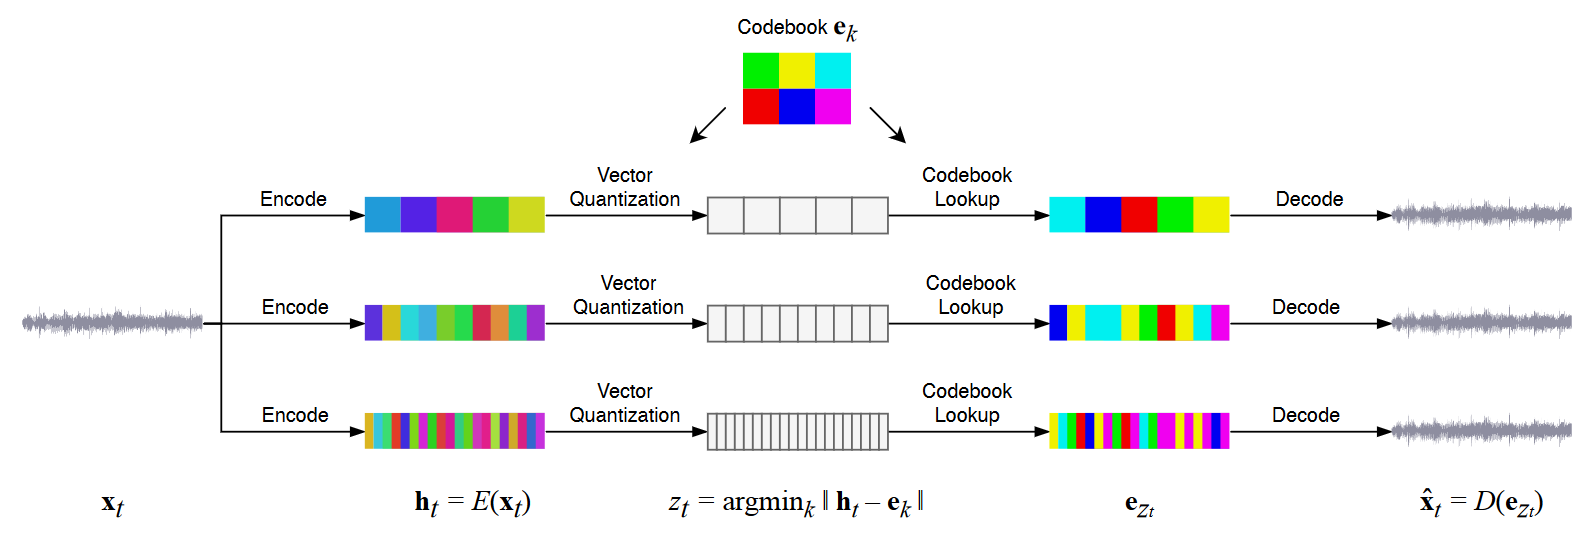
\includegraphics[scale=0.2]{figure/musicvqvae.png}
    \end{center}

    \begin{itemize}
        \item hierarchical VQ-VAE を使用(\cite{gdhfiv2}\cite{ndrl}で提案されたものを修正)
        \item Encoder/Decoderは複数のCNNで構成
        \item 学習の対象:Encoder, Decoder, Codebook
    \end{itemize}
\end{frame}


\begin{frame}
    \frametitle{Music VQ-VAE}
    \begin{center}
        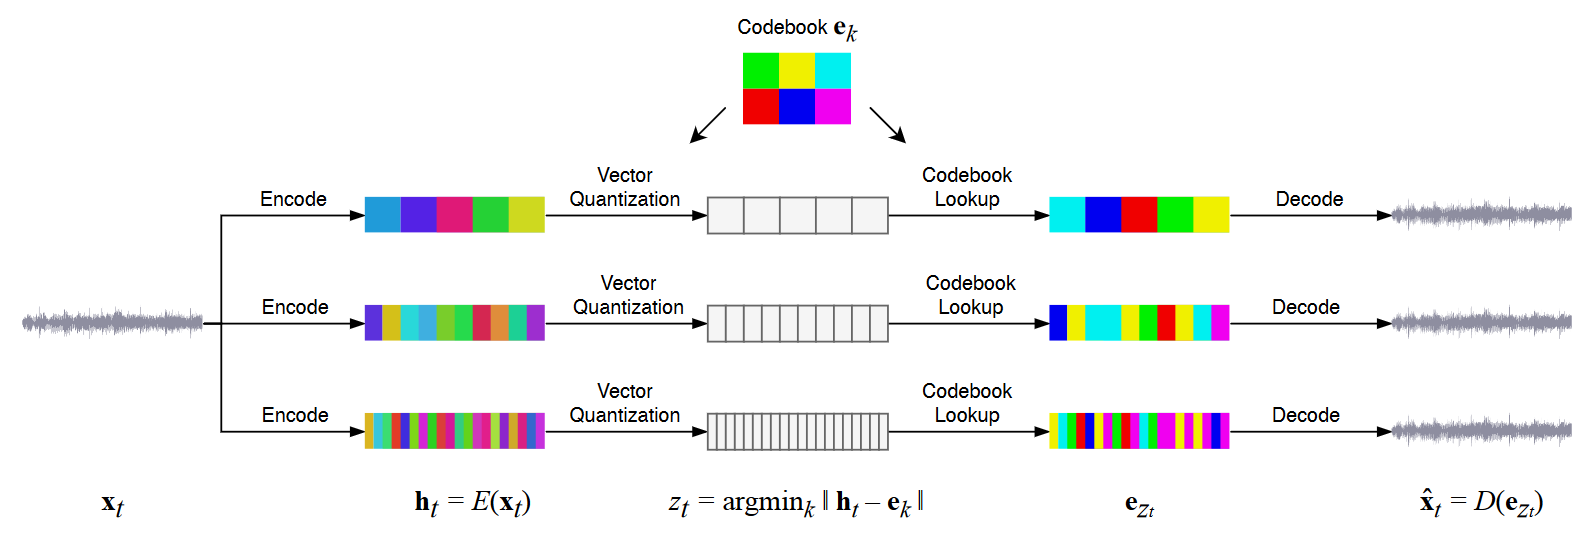
\includegraphics[scale=0.2]{figure/musicvqvae.png}
    \end{center}

    Encodeの流れ
    \begin{enumerate}
        \item 入力$\bm{x}_t$をEncodeして潜在ベクトル$\bm{h}_t = E(\bm{x}_t)$へ
        \item $\bm{h}_t$をベクトル量子化して$z_t = \mathrm{argmin}_k \|\bm{h}_t - \bm{e}_k\|$へ\\
    \end{enumerate}
    \vspace{0.5\baselineskip}

    Codebookが持つ要素$\bm{e}$のうち$\bm{h}$に一番近いもの($\bm{e}_{z_t}$)を見つける\\
    ここで現れる$z$が楽曲の離散表現($z$はcodeと呼ばれる)
\end{frame}


\begin{frame}
    \frametitle{Music VQ-VAE}
    \begin{center}
        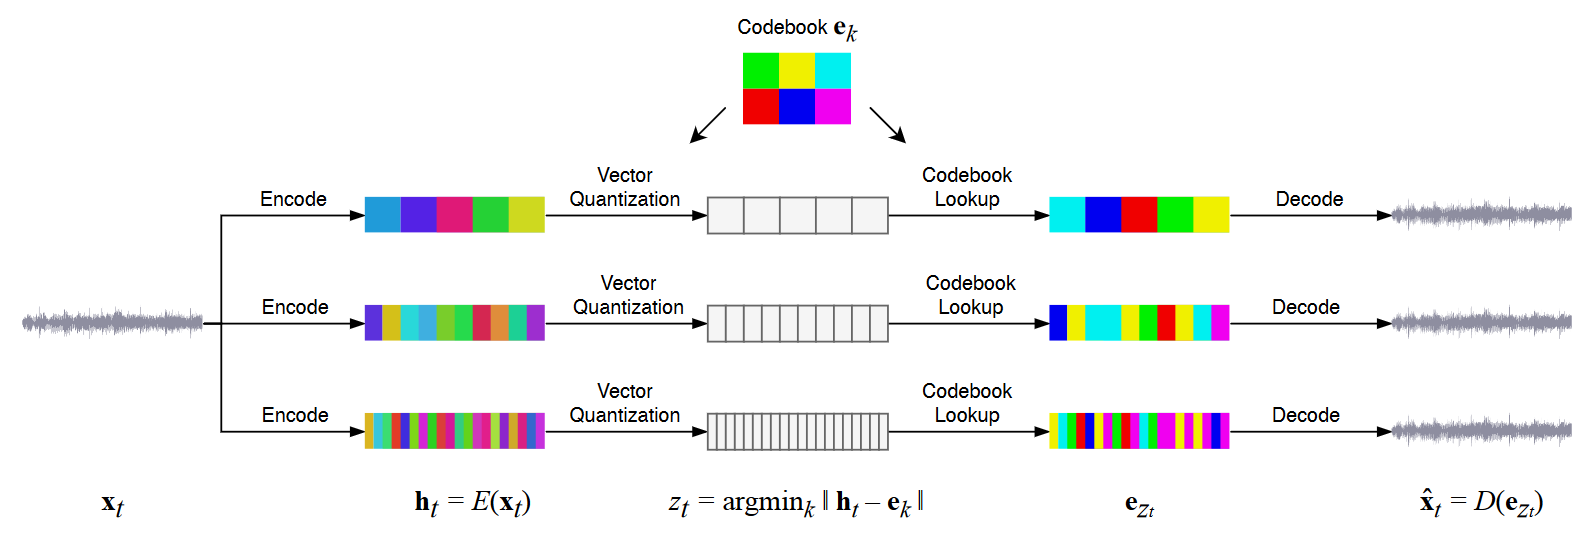
\includegraphics[scale=0.2]{figure/musicvqvae.png}
    \end{center}

    Decodeの流れ
   \begin{enumerate}
       \item codebookを参照してcode $z_t$をベクトル$\bm{e}_{z_t}$へ
       \item $\bm{e}_{z_t}$をDecodeして入力を復元$\hat{\bm{x}_{t}} = D(\bm{e}_{z_t})$
   \end{enumerate}
\end{frame}


\begin{frame}
    \frametitle{Music VQ-VAE}
    \begin{center}
        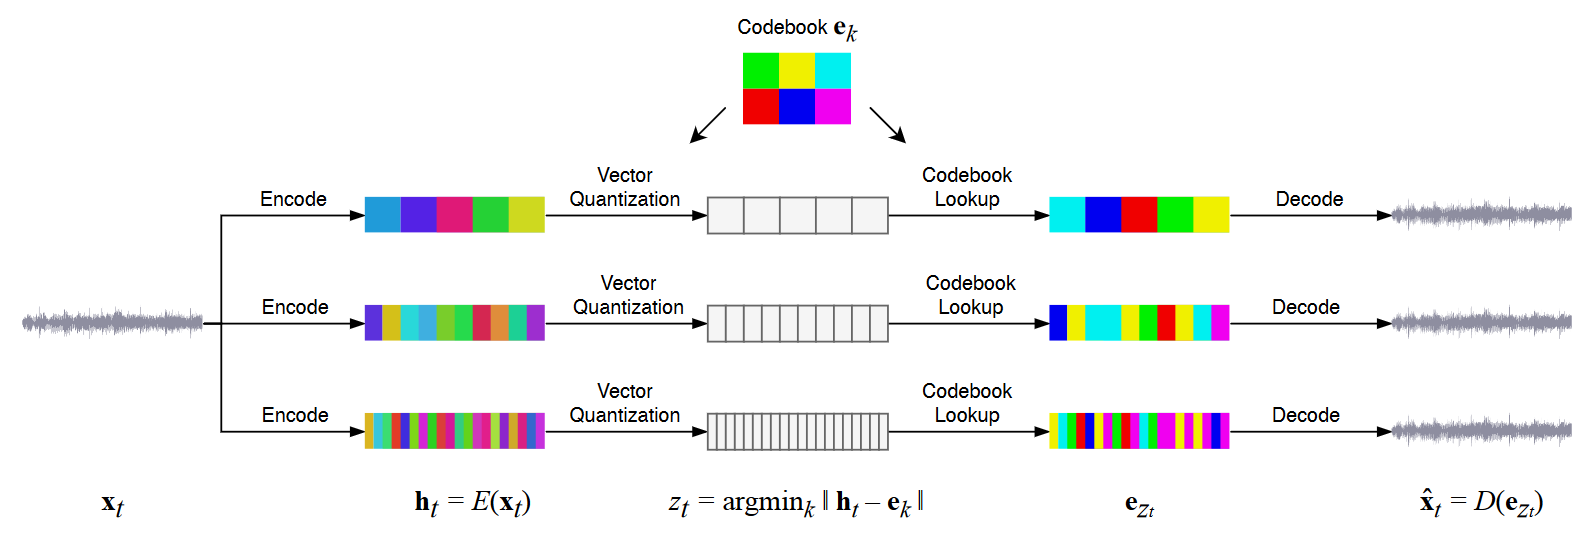
\includegraphics[scale=0.2]{figure/musicvqvae.png}
    \end{center}

    \begin{itemize}
        \item Top/Middle/Bottomで圧縮率を変える
        \item 上にあがるにつれて抽象度は高くなる
        \item 抽象度によってよりlocal/globalな情報を捉える
    \end{itemize}
\end{frame}


\begin{frame}
    \frametitle{Music VQ-VAE}
    Objective
    \begin{align}
        \mathcal{L} &= \mathcal{L}_{\mathrm{recons}} + \mathcal{L}_{\mathrm{codebook}} + \beta \mathcal{L}_{\mathrm{commit}}\\
        \mathcal{L}_{\mathrm{recons}} &= \frac{1}{T} \sum_{t} \| \bm{x}_t - D(\bm{e}_{z_t})\|_2^2\\
        \mathcal{L}_{\mathrm{codebook}} &= \frac{1}{S} \sum_{s} \| \mathrm{sg}\left[\bm{h}_s\right] - \bm{e}_{z_t} \|_2^2\\
        \mathcal{L}_{\mathrm{commit}} &= \frac{1}{S} \sum_{s} \| \bm{h}_s - \mathrm{sg}\left[\bm{e}_{z_s}\right] \|_2^2
    \end{align}
    (記号)$\mathrm{sg}$ (stop-gradient operation):逆伝播のとき勾配を0にする
    \vspace{\baselineskip}

    各項の役割
    \begin{itemize}
        \item[(2)] 入力$\bm{x}$と出力$\hat{\bm{x}}=D(\bm{e}_z)$を近づける
        \item[(3)] codebookが持つ要素$\bm{e}_z$と潜在ベクトル$\bm{h}$を近づける
        \item[(4)] 潜在ベクトル$\bm{h}$が動きすぎるのを防ぐ ($\beta=0.02$は重み)
    \end{itemize}
\end{frame}


\begin{frame}
    \frametitle{Music VQ-VAE}
    codebookの更新
    \vspace{\baselineskip}

    Exponential Moving Average {(\footnotesize \cite{ndrl}より)}
    \begin{itemize}
        \item $\{ z_{i,1}, \ldots , z_{i,n_i}\}$:$\bm{e}_i$に最も近い$n_i$個のEncoderの出力から成る集合
        \item $\gamma \in \left[0, 1\right]$ :decay parameter ($\gamma = 0.99$)
    \end{itemize}
    \begin{align*}
        N_{i}^{(t)} &\coloneqq N_{i}^{(t-1)} \ast \gamma + n_{i}^{(t)} (1-\gamma) \\
        m_{i}^{(t)} &\coloneqq m_{i}^{(t-1)} \ast \gamma + \sum_{j} z_{i,j}^{(t)} (1-\gamma) \\
        e_{i}^{(t)} &\coloneqq \frac{m_{i}^{(t)}}{N_{i}^{(t)}}
    \end{align*}
\end{frame}


\begin{frame}
    \frametitle{Music VQ-VAE}
    \begin{center}
        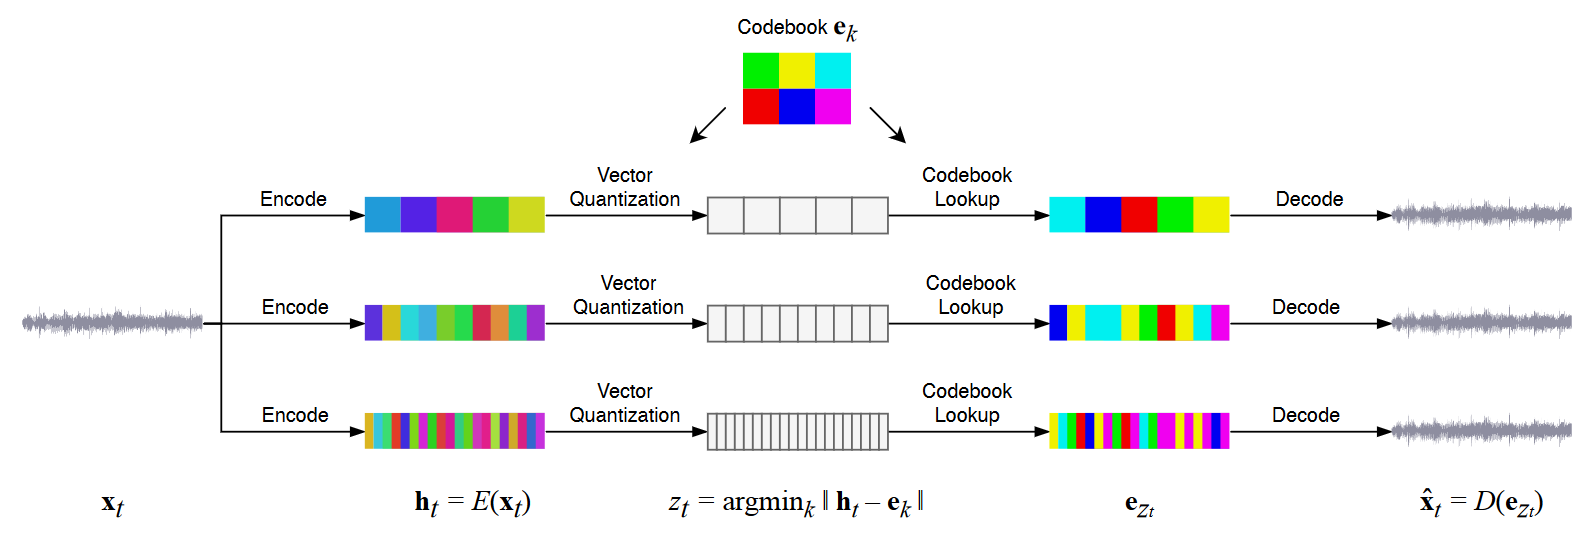
\includegraphics[scale=0.20]{figure/musicvqvae.png}
    \end{center}

    (1) Random restarts for embeddings
    \begin{itemize}
        \item 問題点:codebook collapse \\
        Codebook内の一部のベクトルしか使われない
        \item 解決策:random restart \\
        codebook内のベクトルの平均使用量が閾値以下になると,そのベクトルをrandomに選んだEncoderの出力の一つにreset
    \end{itemize}
\end{frame}


\begin{frame}
    \frametitle{Music VQ-VAE}
    \begin{center}
        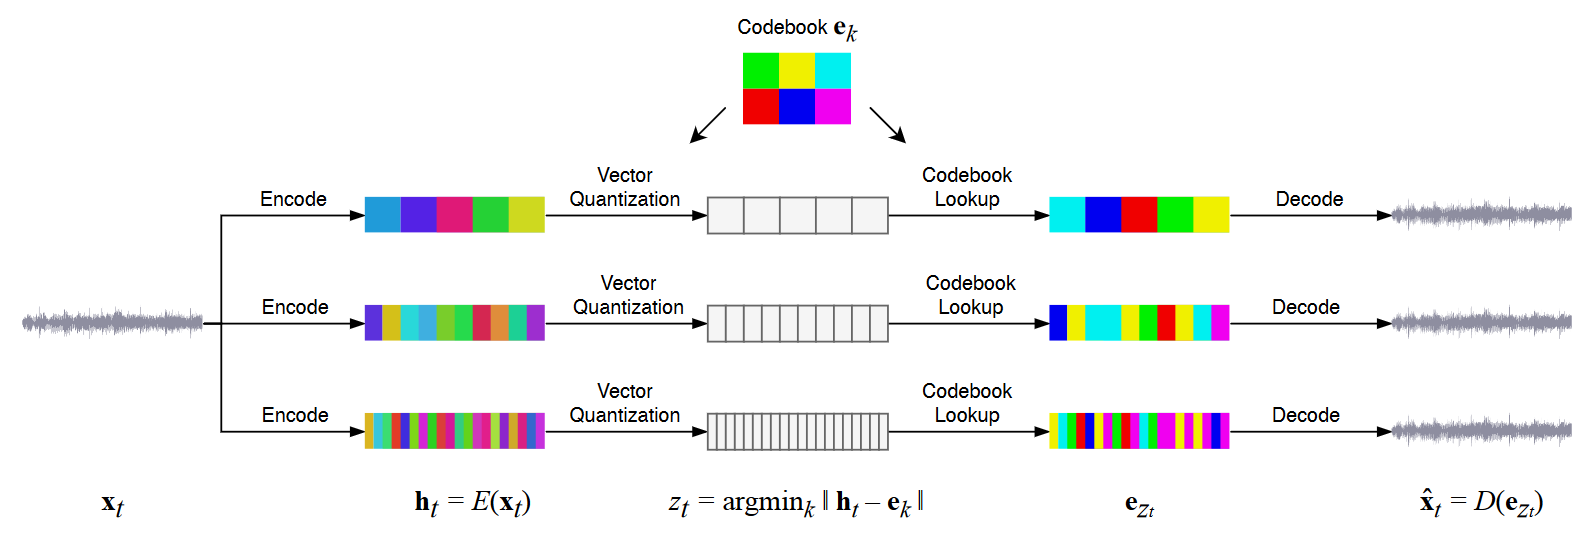
\includegraphics[scale=0.20]{figure/musicvqvae.png}
    \end{center}

    (2) Separated Autoencoders
    \begin{itemize}
        \item 問題点:a complete collapse \\
        top levelがほとんど使われない
        \item 解決策:各レベルのEncoderを別々に学習
    \end{itemize}
\end{frame}


\begin{frame}
    \frametitle{Music VQ-VAE}
    \begin{center}
        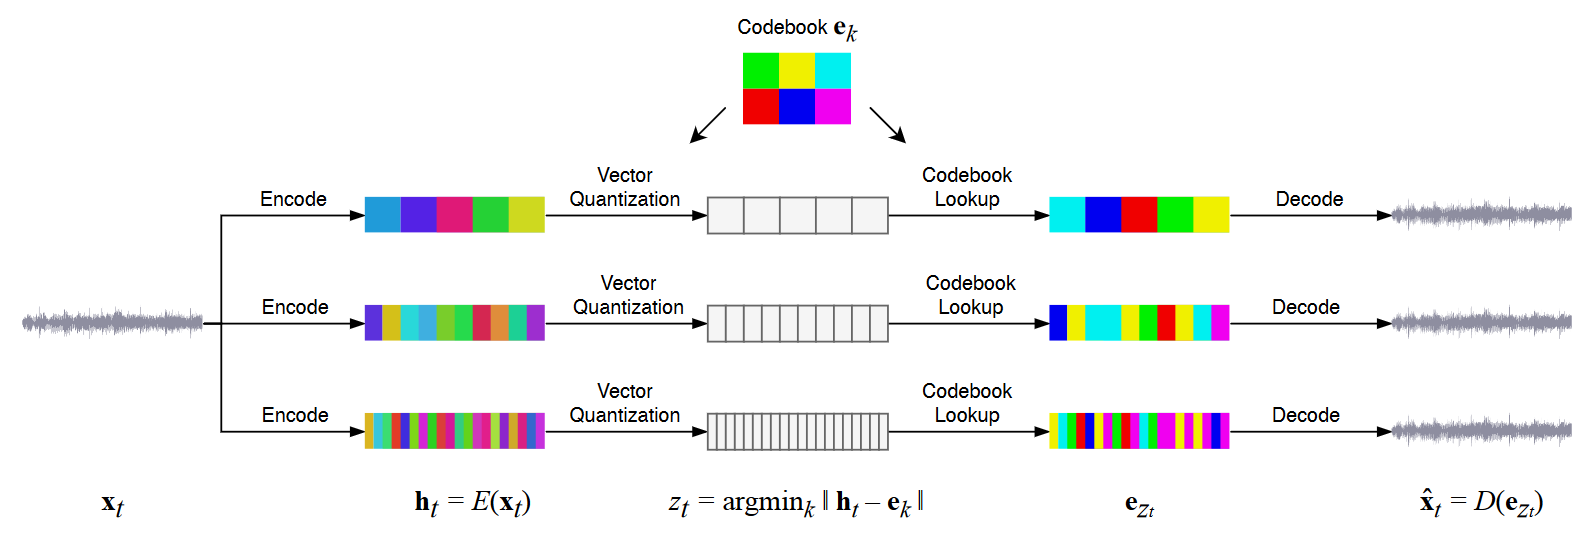
\includegraphics[scale=0.20]{figure/musicvqvae.png}
    \end{center}

    (3) Spectral loss
    \begin{itemize}
        \item 問題点:モデルが低周波数のみを学習
        \item 解決策:Spactral lossの導入
    \end{itemize}
    \begin{align*}
        \mathcal{L}_{\mathrm{spec}} = \| \, | \mathrm{STFT}(\bm{x}) | - | \mathrm{STFT}(\hat{\bm{x}}) | \, \|_2
    \end{align*}
\end{frame}


\begin{frame}
    \frametitle{Music Prior and Upsamplers}
    (VQ-VAEの学習後)
    \vspace{\baselineskip}

    prior $p(\bm{z})$ をモデル化
    \begin{align}
        p(\bm{z}) &= p(\bm{z}^{\mathrm{top}}, \bm{z}^{\mathrm{middle}}, \bm{z}^{\mathrm{bottom}}) \\
        &= p(\bm{z}^{\mathrm{top}}) p(\bm{z}^{\mathrm{middle}} | \bm{z}^{\mathrm{top}}) p(\bm{z}^{\mathrm{bottom}} | \bm{z}^{\mathrm{middle}}, \bm{z}^{\mathrm{top}})
    \end{align}

    \begin{itemize}
        \item $p(\bm{z}^{\mathrm{top}})$ : Top-Level Prior
        \begin{itemize}
            \item 条件より$\bm{z}^{\mathrm{top}}$を生成
        \end{itemize}
        \vspace{0.5\baselineskip}
        \item $p(\bm{z}^{\mathrm{middle}} | \bm{z}^{\mathrm{top}})$ : Middle Upsampler
        \begin{itemize}
            \item 条件と$\bm{z}^{\mathrm{top}}$より$\bm{z}^{\mathrm{middle}}$を生成
        \end{itemize}
        \vspace{0.5\baselineskip}
        \item $p(\bm{z}^{\mathrm{bottom}} | \bm{z}^{\mathrm{middle}}, \bm{z}^{\mathrm{top}})$ : Bottom Upsampler
        \begin{itemize}
            \item 条件と$\bm{z}^{\mathrm{middle}}$より$\bm{z}^{\mathrm{bottom}}$を生成
        \end{itemize}
    \end{itemize}
\end{frame}


\begin{frame}
    \frametitle{Music Prior and Upsamplers}
    \begin{columns}
        %%% figure - left
        \begin{column}[T]{0.50\textwidth}
            \centering
            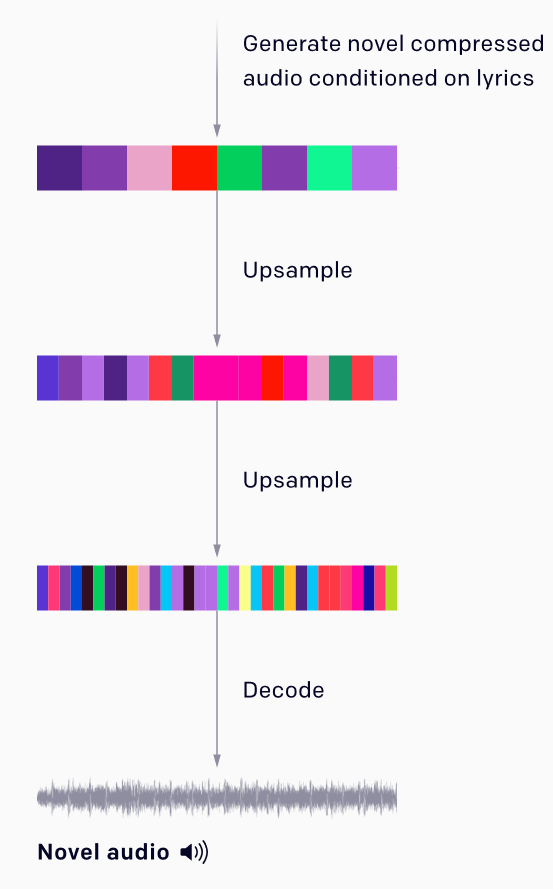
\includegraphics[scale=0.5]{figure/upsampleflow.png}
        \end{column}
        %%% text - right
        \begin{column}[T]{0.50\textwidth}
            Sampleの流れ
            \begin{enumerate}
                \item Lyrics条件をもとにしてTop-Level Priorが$\bm{z}^{\mathrm{top}}$を生成
                \label{flow_toplevel}
                \item \ref{flow_toplevel}で生成された$\bm{z}^{\mathrm{top}}$と条件より$\bm{z}^{\mathrm{middle}}$へupsample
                \label{flow_midupsample}
                \item \ref{flow_midupsample}で生成された$\bm{z}^{\mathrm{middle}}$と条件より$\bm{z}^{\mathrm{bottom}}$へupsample
                \label{flow_bottomupsample}
                \item \ref{flow_bottomupsample}で生成された$\bm{z}^{\mathrm{bottom}}$をVQ-VAEのEncoderに渡す
            \end{enumerate}
            \vspace{\baselineskip}
            Top-Level Prior / UpsamplersはTransformerを基本とした構造
            \vspace{\fill}
            \flushright{\textcolor[gray]{0.7}{{\scriptsize 画像:\url{https://openai.com/blog/jukebox/}}}}
        \end{column}
    \end{columns}
\end{frame}


\begin{frame}
    \frametitle{Music Prior and Upsamplers}
    \begin{center}
        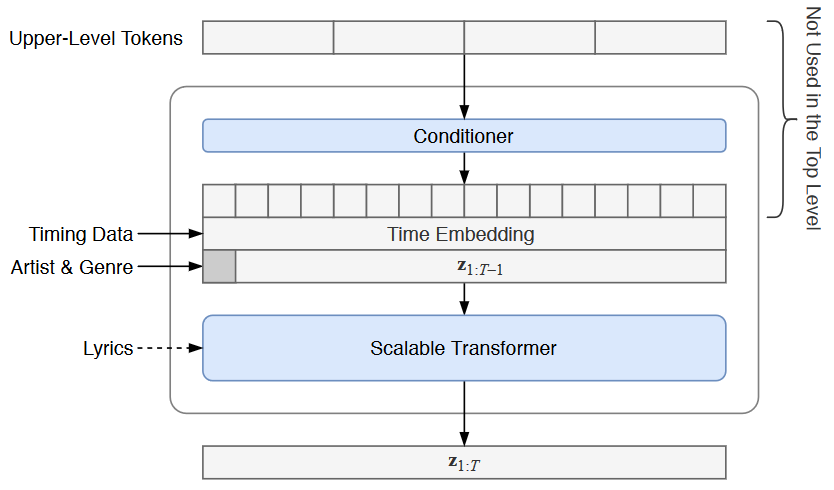
\includegraphics[scale=0.25]{figure/priormodeldetail.png}
    \end{center}
    Top-Level Priorの構造
    \begin{itemize}
        \item Scalable Transformer(Transformerの簡易版)を使用
        \item Artist, Genre, Timing ConditioningをEmbeddingとして与える
        \item Lyrics Conditioningを与える
        \item 既に生成したコード($\bm{z}_{1:T-1}$)より次のコード($\bm{z}_{T}$)を生成
    \end{itemize}
\end{frame}


\begin{frame}
    \frametitle{Music Prior and Upsamplers}
    \begin{center}
        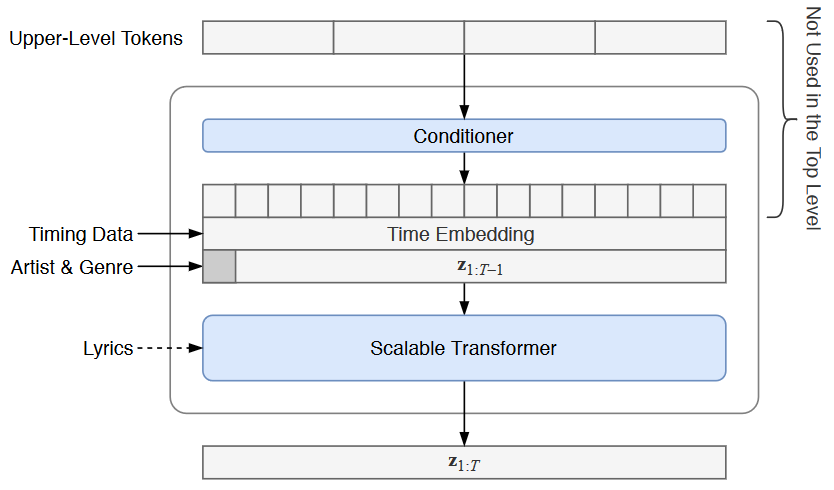
\includegraphics[scale=0.25]{figure/priormodeldetail.png}
    \end{center}
    Upsamplerの構造
    \begin{itemize}
        \item Scalable Transformer(Transformerの簡易版)を使用
        \item Artist, Genre, Timing ConditioningをEmbeddingとして与える
        \item 上位レベルのtokenをConditionerで変換,条件として与える
        \item 既に生成したコード($\bm{z}_{1:T-1}$)より次のコード($\bm{z}_{T}$)を生成
    \end{itemize}
\end{frame}


\begin{frame}
    \frametitle{Music Prior and Upsamplers}
    Top-Level Prior / Upsamplerの学習
    \begin{itemize}
        \item 最尤推定 {\scriptsize (?)}
        \item {\small We use an autoregressive Sparse Transformer trained with maximum-likelihood estimation over this compressed space,and also train autoregressive upsamplers to recreate the lost information at each level of compression.}
        \vspace{\baselineskip}

        \item ConditionerはCNNで構成 {\small (学習方法 ?)}
    \end{itemize}
    \vspace{\baselineskip}

    % Lyrics Conditioning
    % \begin{itemize}
    %     \item 学習時に歌詞とそれに対応するaudio segment(24秒)を与える
    %     \item audioの中に現れる歌詞が不明
    %     \item vocal抽出+alignment(NUS AutoLyricsAlign)で歌詞とaudioの対応付け
    % \end{itemize}
\end{frame}


\begin{frame}
    \frametitle{生成楽曲}
    生成楽曲:\url{https://jukebox.openai.com/}
    \vspace{\baselineskip}

    manuallyに評価
    \begin{itemize}
        \item 生成された楽曲は一貫性があり音楽的
        \item 長期的な構造(コーラスやメロディの繰り返し)は持たない
        \item 歌詞:自然,メロディ:人間の作曲よりは面白くない
        \item モデルは幅広い歌唱スタイルや演奏スタイルを学習
        \item 面白く多様性に富んでいるが、全体的には原曲に比べてまだまだ音楽性に改善の余地がある
    \end{itemize}
\end{frame}


\begin{frame}
    \frametitle{Future Work}
    \begin{itemize}
        \item 音楽的構造
        \begin{itemize}
            \item localな音やハーモニーが常に意味を成す
            \item ニュアンスのある適当な楽器の強弱
            \item 録音バランス,ノイズ
            \item 繰り返されるコーラスやメロディの応答などの長期の音楽的構造
        \end{itemize}
        \vspace{0.5\baselineskip}
        \item 言語・スタイルの多様性
        \begin{itemize}
            \item このモデルは歌詞が英語の曲で学習
            \item 他の言語やアーティストを含める
            \item 創造性や発展は現存のスタイルの普通ではないな融合によって起こる
        \end{itemize}
        \vspace{0.5\baselineskip}
        \item 音楽制作ツールとしての応用 [重要]
        \begin{itemize}
            \item mood/dynamic/楽器の演奏タイミングでの条件付け
            \item 楽曲生成にかかる時間:1分の楽曲生成に9時間程度
            \item top-level tokenを生成した段階でdecode,人間が概要を聞いて気に入ったものを生成
        \end{itemize}
    \end{itemize}
\end{frame}


% \begin{frame}
%     \frametitle{Conclusion}
%     \begin{itemize}
%         \item Jukebox(raw audio musicの生成モデル)の提案
%         \item Hierarchical VQ-VAEの構造により実現
%         \item 生成する音楽の条件付け(アーティスト・ジャンル・歌詞)
%         \item 従来の音楽生成(20-30秒)を遥かに上回る性能(数分)
%         \item 自然な歌声を含む音楽の生成
%     \end{itemize}
% \end{frame}


\begin{frame}
    \frametitle{参考文献}
    \beamertemplatetextbibitems
    % \bibliographystyle{apalike}
    % \bibliographystyle{alpha}
    \bibliographystyle{unsrt}
    \bibliography{jukebox}
 \end{frame}


 % \begin{frame}
 %     \frametitle{}
 % \end{frame}



 \begin{frame}
     \frametitle{Training Details}
     \begin{itemize}
         \item Music VQ-VAE
         \begin{itemize}
             \item audioを8x, 32x, 128xに圧縮
             \item codebookのサイズ:各レベル2048
             \item パラメータ数:2 million
             \item 44.1kHz,9秒のaudio clip:256V100で3日
         \end{itemize}
         \vspace{\baselineskip}
         \item Prior / Upsampler
         \begin{itemize}
             \item パラメータ数:5 billion(Top-Level Prior),1 billion(Upsamplers)
             \item VQ-VAEのtoken 8192個(audio換算で24,6,1.5秒):128V100sで4週間,128V100sで2週間
             \item Lyrics conditioning用のEncoder追加後:512V100sで2週間
         \end{itemize}
     \end{itemize}
 \end{frame}


 \begin{frame}
    \frametitle{Music VQ-VAE}
    \begin{figure}[ht]
        \begin{center}
            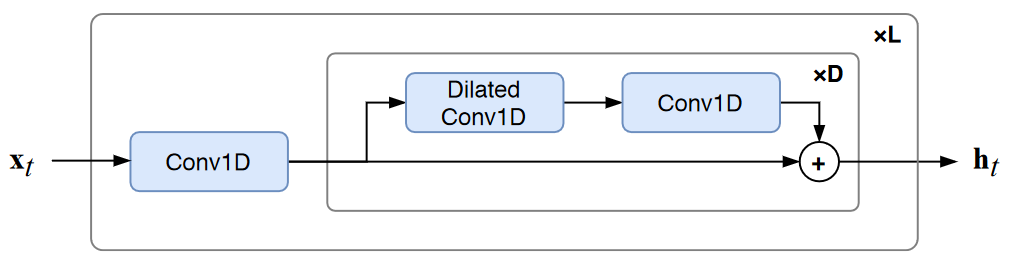
\includegraphics[scale=0.200]{figure/encoder.png}
            \vspace{-0.5\baselineskip}
            \caption{Encoder}
        \end{center}
    \end{figure}
    \vspace{-0.5\baselineskip}

    \begin{figure}[ht]
        \begin{center}
            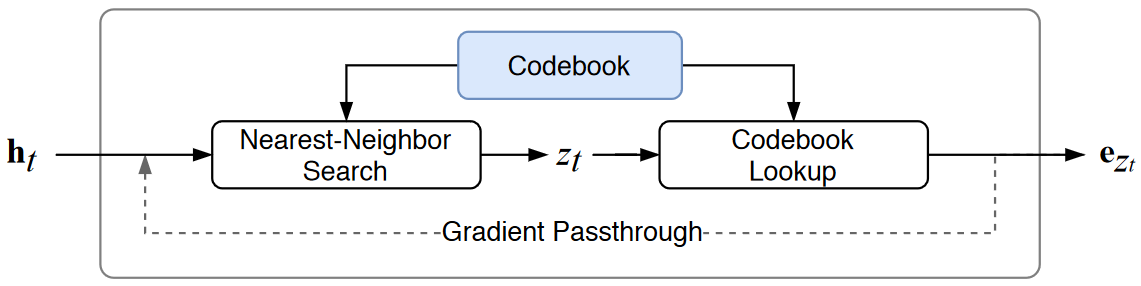
\includegraphics[scale=0.175]{figure/bottleneck.png}
            \vspace{-0.5\baselineskip}
            \caption{Bottleneck}
        \end{center}
    \end{figure}
    \vspace{-0.5\baselineskip}

    \begin{figure}[ht]
        \begin{center}
            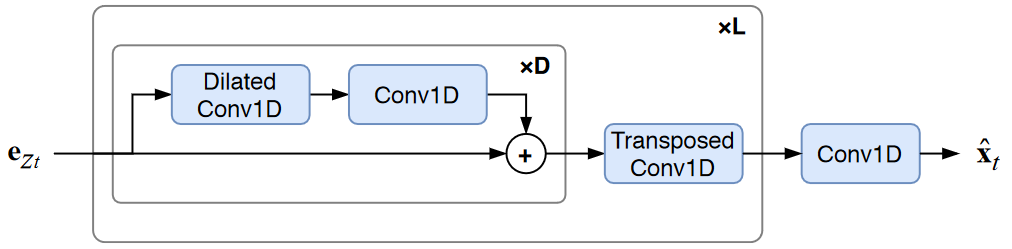
\includegraphics[scale=0.195]{figure/decoder.png}
            \vspace{-0.5\baselineskip}
            \caption{Decoder}
        \end{center}
    \end{figure}
\end{frame}


\begin{frame}
    \frametitle{Music Prior and Upsamplers}
    \begin{columns}
        %%% figure - left
        \begin{column}[T]{0.60\textwidth}
            \begin{figure}
                \begin{center}
                    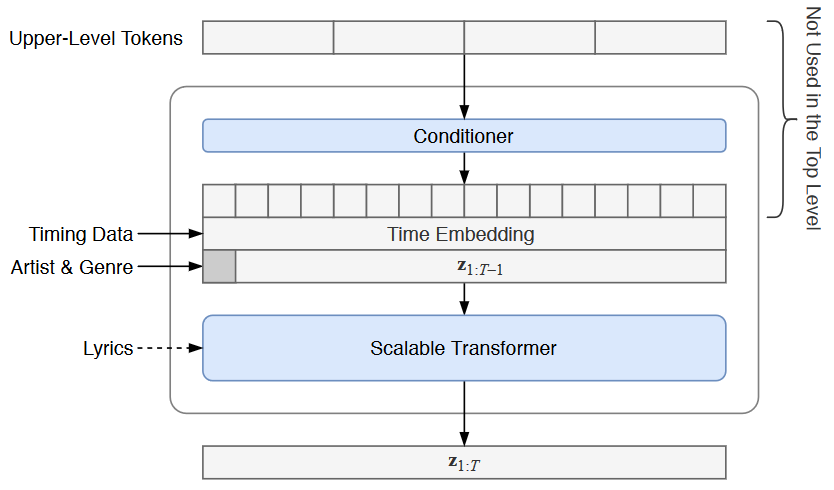
\includegraphics[scale=0.2]{figure/priormodeldetail.png}
                    \caption{Top-Level Prior / Upsamplers}
                \end{center}
            \end{figure}
        \end{column}
        %%% text - right
        \begin{column}[T]{0.40\textwidth}
            \begin{figure}
                \begin{center}
                    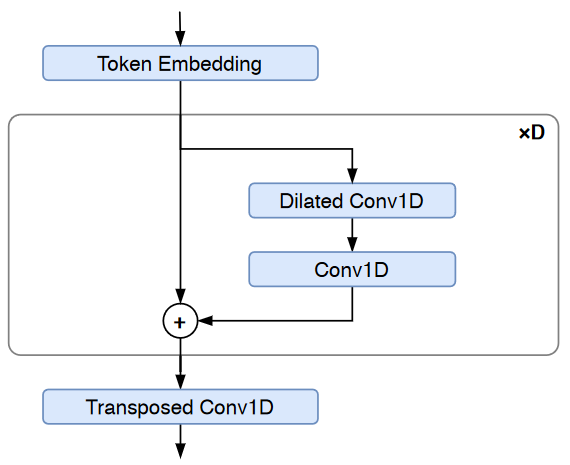
\includegraphics[scale=0.2]{figure/conditionerdetail.png}
                    \caption{Conditioner}
                \end{center}
            \end{figure}
        \end{column}
    \end{columns}
\end{frame}


% \begin{frame}
%     \frametitle{Music Prior and Upsamplers}
%     \begin{columns}
%         %%% figure - left
%         \begin{column}[c]{0.50\textwidth}
%             \begin{center}
%                 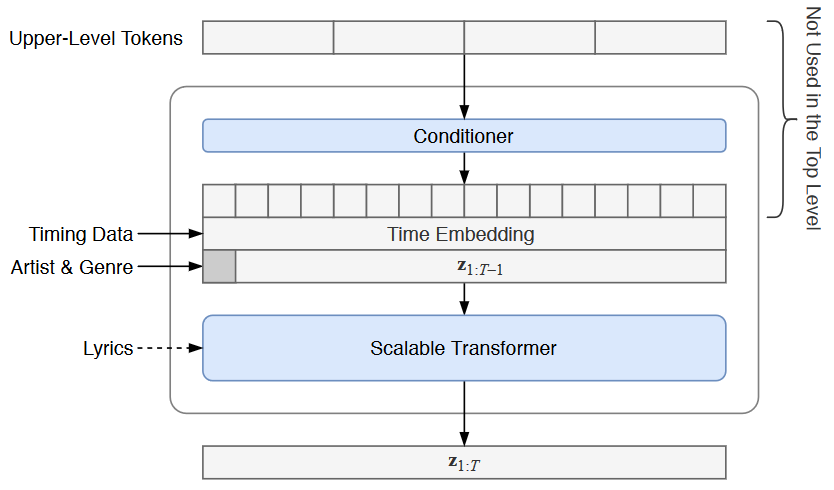
\includegraphics[scale=0.18]{figure/priormodeldetail.png}
%             \end{center}
%         \end{column}
%         %%% text - right
%         \begin{column}[c]{0.50\textwidth}
%             \begin{center}
%                 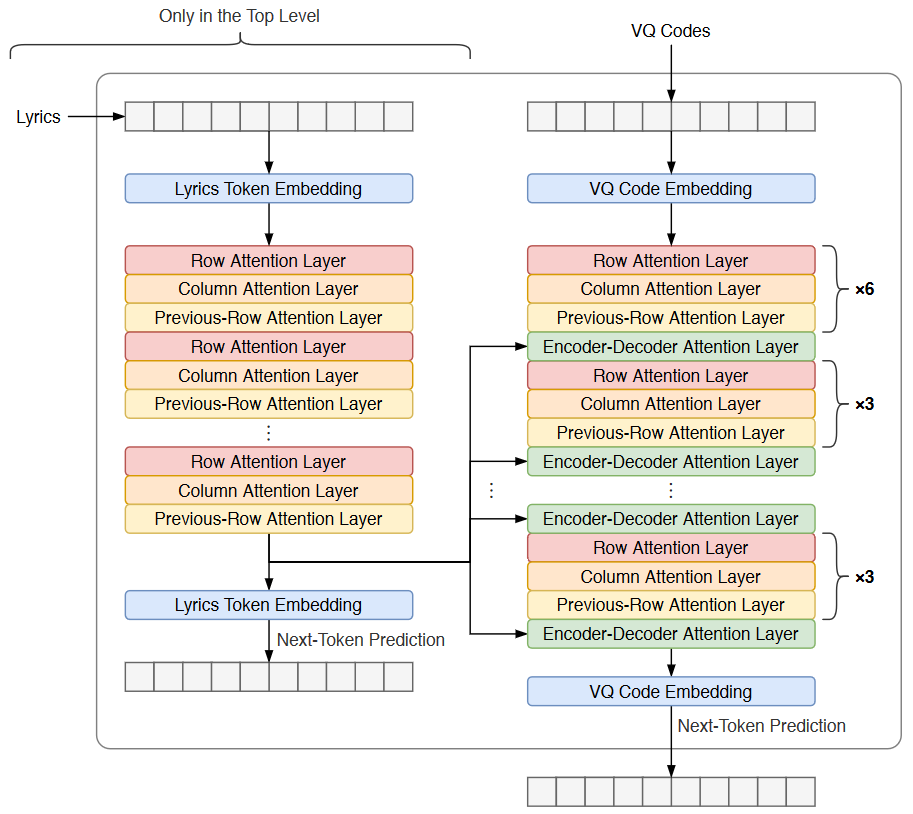
\includegraphics[scale=0.16]{figure/scalabletransformerarchitecture.png}
%             \end{center}
%         \end{column}
%     \end{columns}
%
%     Lyrics Conditioning  %%% TODO!!!!
%     \begin{itemize}
%         \item encoder-decoder形式のモデル
%         \item Top-Level PriorにEncoderを付け加える形
%         \item {\small The lyrics encoder is a Transformer with an autoregressive modeling loss for lyrics (?)}
%     \end{itemize}
% \end{frame}


\begin{frame}
    \frametitle{Music Prior and Upsamplers}
    \begin{columns}
        %%% figure - left
        \begin{column}[T]{0.60\textwidth}
            \begin{figure}
                \begin{center}
                    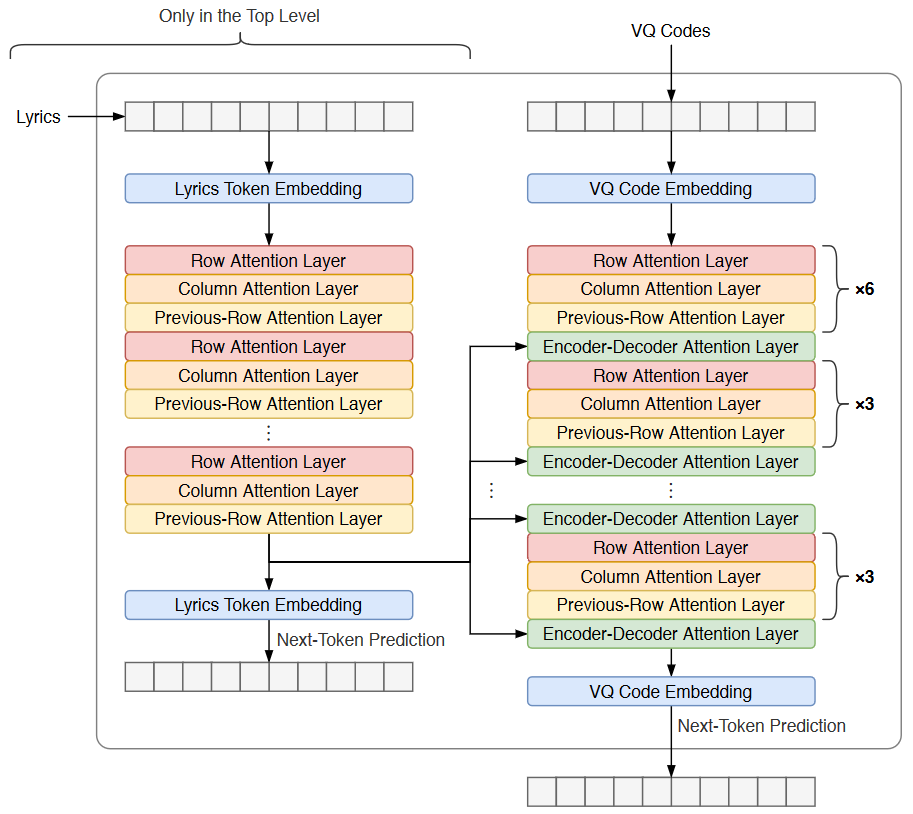
\includegraphics[scale=0.2]{figure/scalabletransformerarchitecture.png}
                    \caption{Scalable Transformer}
                \end{center}
            \end{figure}
        \end{column}
        %%% text - right
        \begin{column}[T]{0.40\textwidth}
            Scalable Transformerの構造
            \vspace{\baselineskip}

            (Top-Level)
            \begin{itemize}
                \item encoder-decoder形式
                \item decoder部はTop-Level Priorを再利用
                \item encoder部にmodel surgeryを使用しdecoder部と合わせる
                \item encoderはLyricsの表現をdecoder部に渡す
            \end{itemize}
            \vspace{\baselineskip}

            (Upsamplers)
            \begin{itemize}
                \item decoder部のみ
            \end{itemize}
        \end{column}
    \end{columns}
\end{frame}


\begin{frame}
    \frametitle{VQ-VAE Ablations}
    \begin{figure}
        \begin{center}
            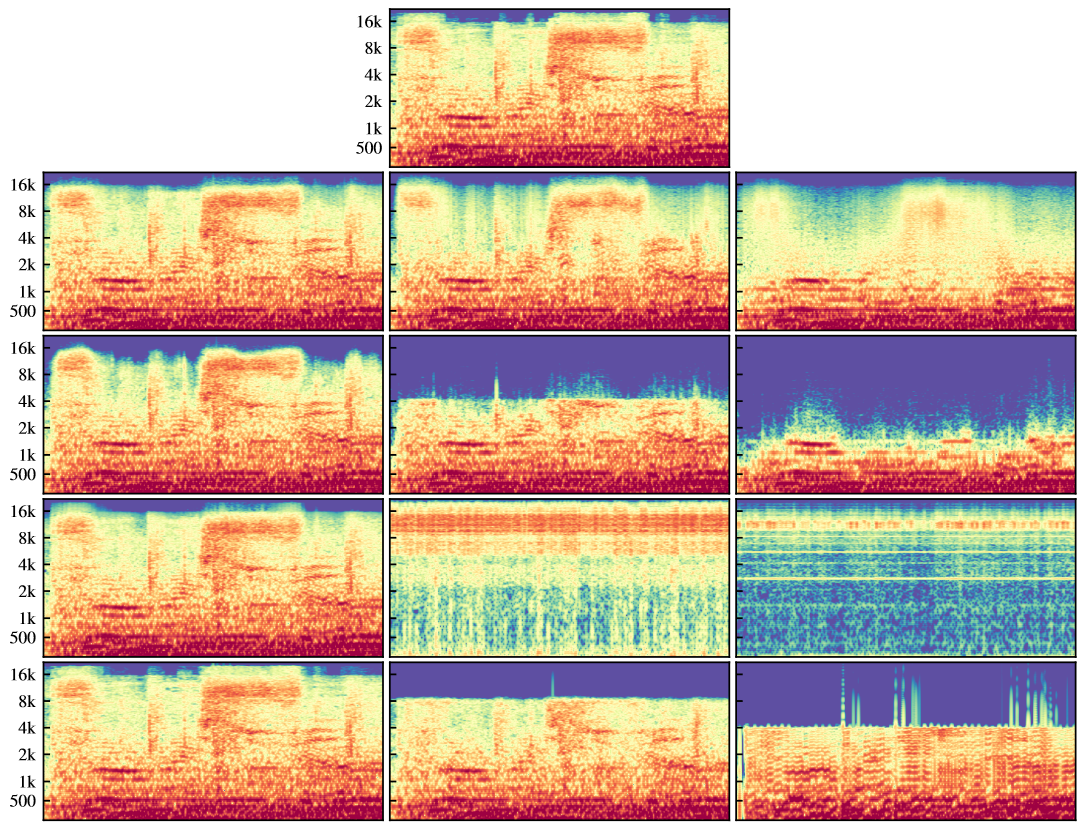
\includegraphics[scale=0.15]{figure/vqvaeablations.png}
            \vspace{-0.5\baselineskip}
            \caption{VQ-VAE再構成比較}
        \end{center}
    \end{figure}
    \begin{itemize}
        \item[軸:] $x$: 時間 (time),$y$: 周波数 (frequency)
        \item[列:] 左から順にbottom, middle, top-levelの再構成
        \item[行:] 1: ground truth, 2: 提案手法, 3: 提案手法(spectral lossなし),\\
        4: VQ-VAE(Separateなし), 5: baseline手法(Opus codec)
    \end{itemize}
\end{frame}



\end{document}
